\input{style/sqtbeamer.tex}

\title{How to Count}
\subtitle{Combinatorics Revisited}
\institute{Sydney Quant Traders}
\date{}

\begin{document}

\maketitle

%%-----------------EAMON
\section{Fundamentals}

\begin{frame}{Counting Problem Examples}
  \begin{itemize}
    \item How many outfits can be made from 4 shirts and 3 hats?
    \item How many ways to arrange 4 people on a circular table?
    \item How many ways to choose a set of 3 cards out of a deck?
    \item How many ways to divide 10 students into 3 teams of non-zero size?
    \item How many bracelets can be made with 3 white and 3 black beads?
    \item How many colorings of a graph with the colors \{red, green, blue\}
    such that no edge connects two vertices of the same color.
  \end{itemize}
\end{frame}

\begin{frame}{Introductory Problem}
  \textcolor{sqt-question}{
    \textbf{Example:} How many outfits can be made from 4 shirts and 3 hats?}\\
  Count the number of ways to construct/configure an outfit.\\
  Each step of the construction/configuration process requires a \textbf{decision}.\\
  \begin{center}
    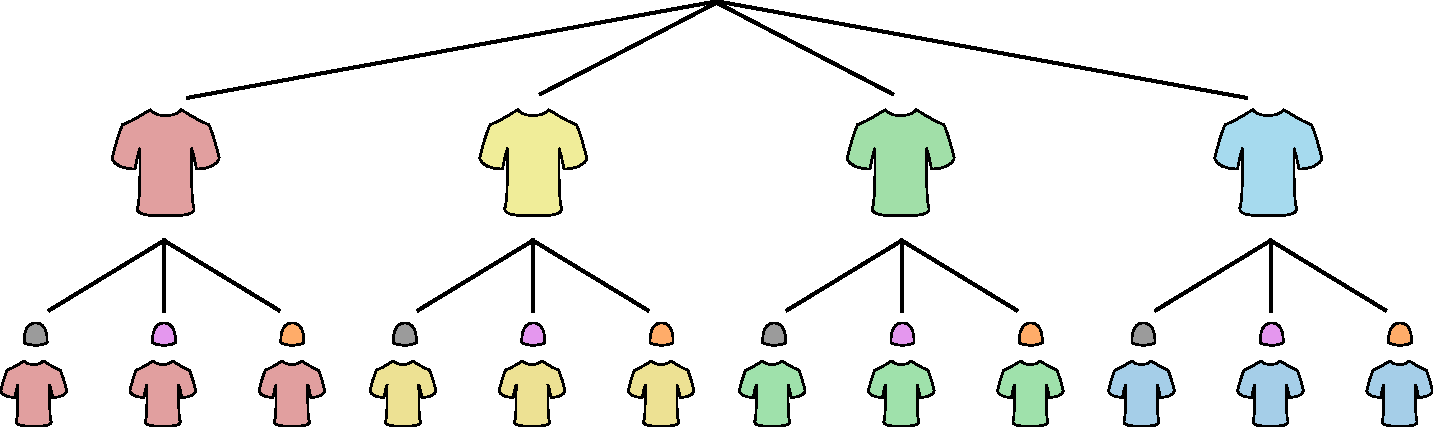
\includegraphics[width=13cm]{assets/outfits.pdf}
  \end{center}
\end{frame}

\begin{frame}{Configuration}
  \begin{sqt:definition}[\textbf{Definition:} configuration]
    A configuration is a way (i.e. sequence of decisions) to construct an object.
  \end{sqt:definition}

  Each leaf node in a decision tree corresponds to a different configuration.

  \begin{center}
    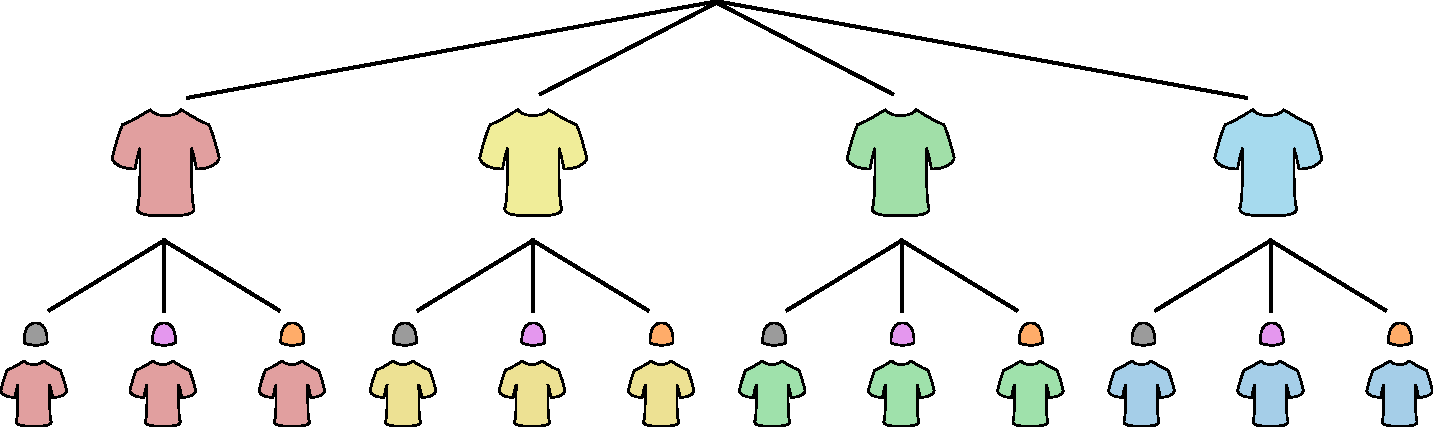
\includegraphics[width=10cm]{assets/outfits.pdf}
  \end{center}
\end{frame}

%%would be cool if you could explain in a similar fashion to http://youtube.com/watch?v=ggNeQUe1Hj8

%TO FINISH
\begin{frame}{Addition and Multiplication}
  example
\end{frame}

\begin{frame}{Exponentiation}
  example
\end{frame}

\begin{frame}{Exponentiation}
  example
\end{frame}

\begin{frame}{Permutations and Combinations}
  example
\end{frame}

\begin{frame}{Stars and Bars}
  example
\end{frame}

%--------------------------------------ADI
\begin{frame}{When Counting Goes Wrong}
  Sometimes we count the same object multiple times.

  \textbf{Example:}
  Circular arrangements

  \begin{itemize}
    \item Rotating a seating arrangement does not create a new arrangement
  \end{itemize}

  \textbf{Problem:}
  \begin{itemize}
    \item Our counting method overcounts
  \end{itemize}

  \textbf{Solution:}
  \begin{itemize}
    \item Group equivalent configurations together
  \end{itemize}
\end{frame}

\section{Foundational Concepts}
\begin{frame}{Equivalence Relation}
  \textcolor{sqt-question}{
    \textbf{Example:} How many ways to arrange 3 people on a circular table?\\
    Two arrangements are identical if one can be obtained
    from the other by rotation.
  }

  \begin{center}
    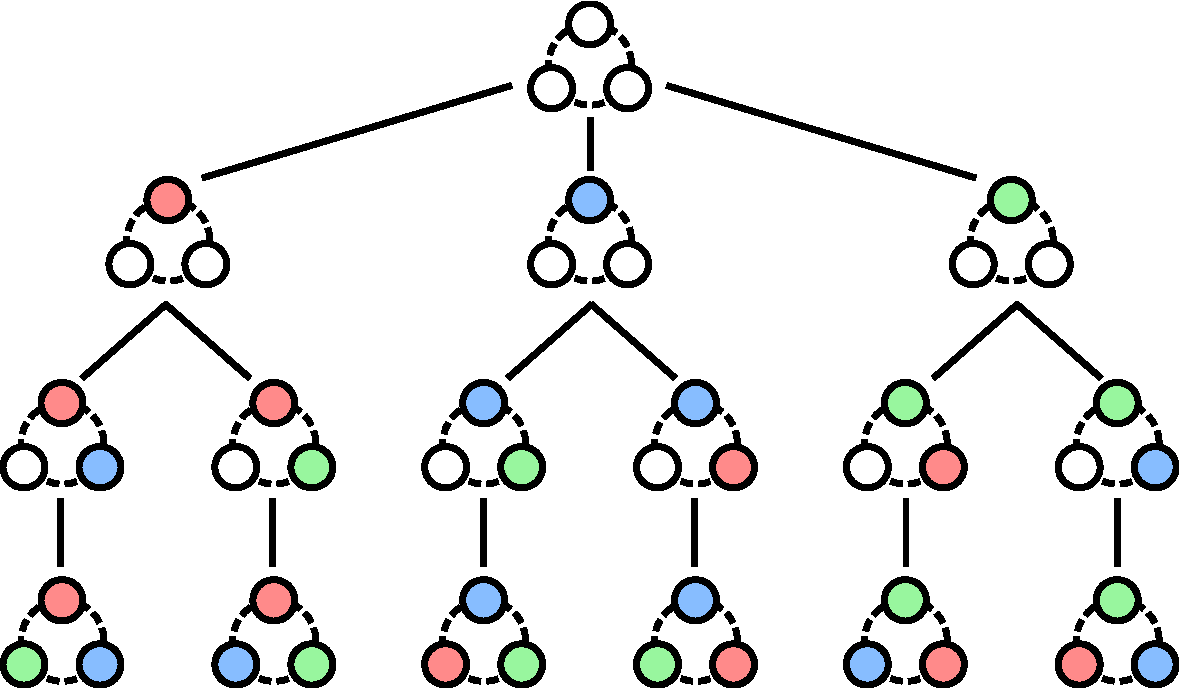
\includegraphics[width=9cm]{assets/circular_seating.pdf}
  \end{center}
\end{frame}

\begin{frame}{Equivalence Relations}
  Let $X$ be the set of configurations.
  A counting quesiton may specify what it means for two configurations $x_1, x_2\in X$ to be considered equal.\\
  In other words, it provides an equivalence relation on the set $X$ of configurations.

  \begin{sqt:definition}[\textbf{Definition:} equivalence relation]
    A binary operator $\sim$ such that the expression $x_1\sim x_2$
    evaluates to $\mathrm{TRUE}$ if $x_1$ should be considered equivalent to $x_2$
    in the context of the counting problem.
  \end{sqt:definition}
  \begin{itemize}
    \item We define when two configurations should be considered "the same"
  \end{itemize}
\end{frame}

\begin{frame}{Equivalence Class}
  \begin{sqt:definition}[\textbf{Definition:} equivalence class]
    The equivalence class of $x$ under $\sim$ is denoted by $[x]_\sim$.\\
    It is defined as the set of all elements equivalent to $x$ under $\sim$.
  \end{sqt:definition}

  \begin{center}
    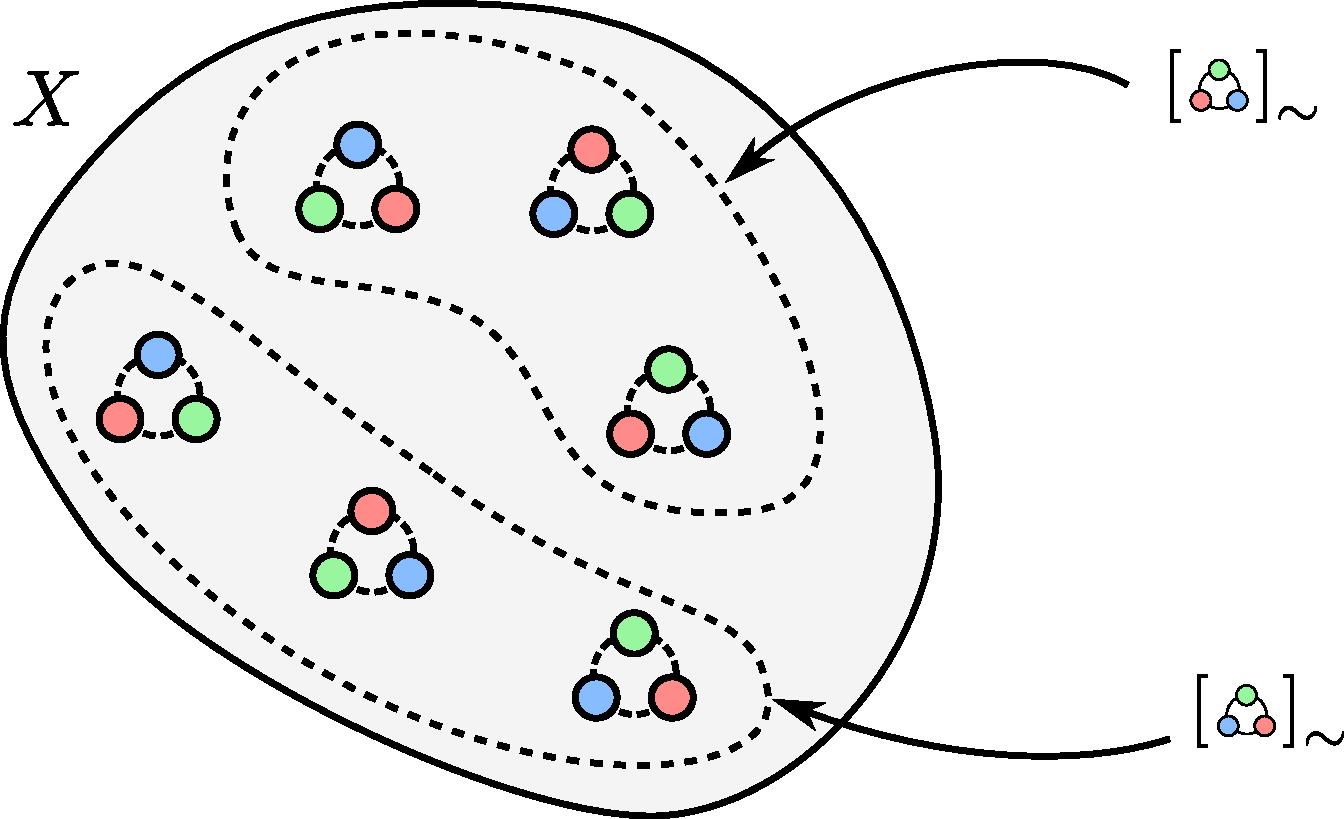
\includegraphics[width=7cm]{assets/equivalence_classes.pdf}
  \end{center}

\end{frame}

\begin{frame}{Quotient Set}
  \begin{sqt:definition}[\textbf{Definition:} quotient set]
    The quotient set of $X$ under $\sim$ is denoted by $X/\sim$.\\
    It is defined as the set of all equivalence classes (under $\sim$) of its elements.
  \end{sqt:definition}

  \begin{center}
    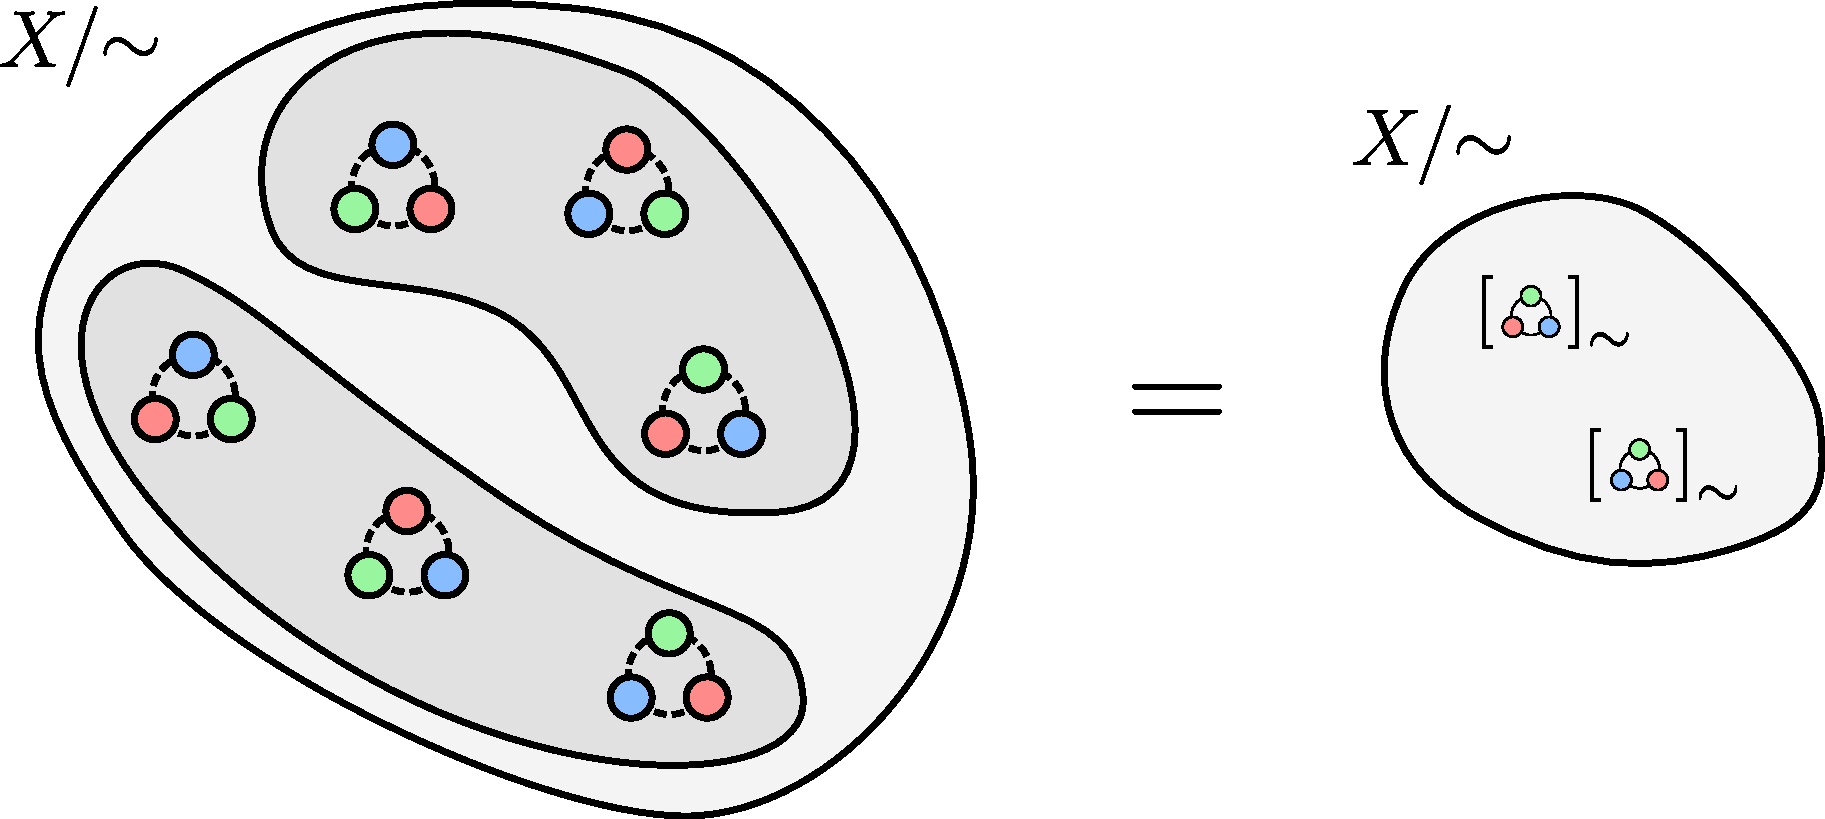
\includegraphics[width=9cm]{assets/quotient.pdf}
  \end{center}
\end{frame}

\section{Group Actions}
\begin{frame}{Group Actions}
  \begin{sqt:definition}[Definition: Action]
    An action on a configuration $x \in S$ is a "movement"(or symmetry) that maps one configuration to another.
  \end{sqt:definition}
  \textbf{Example:} denote $g_1, g_2, g_3 $ to be the actions that rotate a configuration clockwise $0,120,240$ degrees.\\
  \begin{center}
    %insert image consisting of a configuration, its first rotation, its second rotation.
  \end{center}
  Notice we can combine group actions $g_2 \circ g_3 = g_1 $\\
\end{frame}

\begin{frame}{Group Actions}
  \begin{sqt:definition}[Definition:A Group of Actions]
    A set of actions can be considered a group if it obeys the following\\
    \begin{itemize}
      \item The set has to have the "do nothing" action (identity)\\
      \item Composing any two actions must produce an action that is in the set(closure)\\
      \item For an action in the set, there must also be the action that undoes it in the set(Inverse)\\
      \item Composing actions must be associative. so from before $g_2 \circ (g_3 \circ g_1) = (g_2 \circ g_3) \circ g_1  $\\
    \end{itemize}

  \end{sqt:definition}

\end{frame}


% script notes: In not all instances will we find the do nothing action the only action leaving things unchanged
\begin{frame}{What is a Fix}

  \begin{sqt:definition}[\textbf{Definition:} Fix]
    For a set of group actions $G$ acting on $S$, A fix of an action $g \in G$, is
    the set of all elements $s\inS$ that \textbf{remain unchanged} after g is applied.
  \end{sqt:definition}
  This set of elements is denoted by $fix(g)$

  In our example the only action that leaves a configuration unchanged is the "do nothing" action.


\end{frame}

\begin{frame}{Back to the Example}
  \textcolor{sqt-question}{
    \textbf{Example:} How many ways to arrange 3 people on a circular table?
  }

  We can systematically answer this example.

  In our configurations, what arrangements are considered equivalent with an "action"?\\
  What is the size of the quotient set under this equivalence?\\

  Note that it is a coincidence that the equivalence classes are of equal size.
\end{frame}

\begin{frame}{Counting Problems}
  This is a specific example of a general counting problem that we can generalise with the definition.

  \begin{sqt:definition}[Definition: counting problem]
    Determining the size of the quotient set of a specified set $X$ of configurations,
    modulo some specified equivalence relation $\sim$.
  \end{sqt:definition}
\end{frame}

\begin{frame}{Back to the Example}
  \textcolor{sqt-question}{
    \textbf{Example:} How many ways to arrange 3 people on a circular table?\\
  }
  Through the circular arrangement forumula we know there are (2-1)! many ways.\\
  However from a more formal lense we can observe the following\\

  \begin{itemize}
    \item Our set of items that actions happen are all the configurations we listed in our tree. There are 6 of these.
    \item Under our idea of equivalence there are the group actions, $g_1,g_2, g_3$.\\
    \item each group $fix(g_i)$ is an empty set except for the fix of $g1$. who's size is 6.
    \item the average size of the fixes under our equivalence is also 2!
  \end{itemize}


\end{frame}

\begin{frame}{Burnside's Lemma}
  \begin{sqt:definition}[Definition: Burnside's Lemma]
    The number of objects modulo equivalence is said to be\\
    $$|S/\sim| = \frac{1}{|G|} \sum_{g \in G} |fix(g)|$$
  \end{sqt:definition}
  Therefore counting the number of seating arrangements from the last example we have,\\
  $$|S/\sim| = \frac{6 + 0 + 0}{3} = 2$$

\end{frame}


\begin{frame}{Circular arrangements with repetition}
  How many bracelets can be made with 3 white and 3 black beads?
\end{frame}

\begin{frame}{Circular arrangements with repetition}
  We can start off by listing the following features of the problem
  \begin{itemize}
    \item In this example beads of the same color are considered the same.
    \item Two configurations are the equal if they can be rotated into eachother.
    \item Two configurations are also the equal if you can reflect them into eachother.
  \end{itemize}
\end{frame}

\begin{frame}{Circular arrangements with repetition}
  We can set up a decision strucutre to list our our total configurations.\\
  This results in the following configuration.\\

  %insert image of decision tree ( with ...s cuz there are so many)

  Finding the number of ways to arrange 3 black and white beads in a line we have
  $\binom{6}{3} = 20$ such ways. However these do not account for our aforementioned equivalences.

\end{frame}

\begin{frame}{Circular arrangements with repetition}
  We have the following group actions under our equivelance.\\

  we have rotations:
  % 6 such rotations ( r_i)
  we have diagonal reflections:
  % 3 such reflections (rd_i)

  we have edge reflections:
  % 3 such reflections ( re_i)


  Fun fact: this set of group actions is referred to as the dihedral group of order 6, $D_6$.\\

\end{frame}

\begin{frame}{Circular arrangements with repetition}
  With the information established, we can use burnside's lemma.\\
  We shall first observe the fixes of group actions involving rotations.\\
  \begin{itemize}
    \item $g_{60^{\circ}} and g_{300^{\circ}}$ rotate configurations by one left/right.The number of configs that remain\\
    unchanged if this is applied \textbf{is zero.}\\

    \item $g_{120^{\circ}} and g_{240^{\circ}}$ rotate configurations by 2 left/right.\\
    This is fixed by confiugrations with alternating black and white beads, as they repeate at a pattern of every 3 beads.\\
    of which there are \textbf{2 such configurations}. \\
    %insert diagram of these two configurations

    \item $g_{180^{\circ}}$  This rotates configurations by 3. For the config to be the same after rotating by 3, this means\\
    repeating pattern of 3 beads must be in place. This is not possible as 3 black and 3 white beads must exist in the \\
    necklace. Therefore \textbf{no configurations exist}.\\

    item $g_{0^{\circ}}$  This leaves configurations unchanged. the configurations that remain the same once this is applied\\
    are all of them. Therefore \textbf{20 configurations exist}

  \end{itemize}



\end{frame}

\begin{frame}{Circular arrangements with repetition}
  Observing the fixes of group actions involving diagonal reflections.\\
  here are some examples of configurations that are unchanged under reflection.\\
  In each reflection, $rd_i$, the configurations that stay the same must have the same beads across the reflecting line.\\
  The only way to ensure this is if we chose our bipodal nodes to be different so black and white,\\
  of which there are two ways.\\

  we also must arrange the reamaining two nodes along the side, of which there are 2 ways.\\

  Therefore for each reflection there are $2 \times 2 = 4$ such configurations that remain unchanged under it.\\

  therefore $fix(rd_i) = 4$.


\end{frame}

\begin{frame}{Circular arrangements with repetition}
  Observing the fixes of group actions involving edge reflections.\\
  For a reflection to be unchanging it must have the same arrangement of black and white beads across the reflecting line.\\
  by parity since there are an odd number of pairs we cannot have any arrangements that satisfy this.\\
  therefore $fix(re_i) = 0$
\end{frame}

\begin{frame}{Circular arrangements with repetition}
  Now applying burnsides lemma finally we see that,\\

  $$|G/\sim| = frac{1}{|G|} \sigma_{g\in G} fix(g) $$

  $$|G/\sim| = \frac{0+2+2+0+20+4+4+4+0+0+0}{12} =  3$$.

  There are \textbf{only 3 possible} configurations. under rotation, reflection and bead repetition.

\end{frame}

%\begin{frame}{An Example}
%  How many colorings of a graph with the colors \{red, green, blue\}
%  such that no edge connects two vertices of the same color.

%  ...
%\end{frame}

\section{ Practical Techniques}

\begin{frame}{The Inclusion Exclusion Principle}
  The principle of inclusion--exclusion is used when a direct count \textbf{overcounts}
  because some configurations violate one or more constraints.



\end{frame}

\begin{frame}{A Doughnut Distribution Problem}
  \textcolor{sqt-question}{
    \textbf{Example:}
    A baker has 6 identical glazed doughnuts to give to 3 kids: Alex, Blake, and Charlie.
  }

  The parent constraints are:
  \begin{itemize}
    \item Alex can receive at most $1$
    \item Blake can receive at most $2$
    \item Charlie can receive at most $3$
  \end{itemize}

  \vspace{0.5em}

  We want the number of integer solutions to
  \[
    a+b+c=6
  \]
  such that
  \[
    a \le 1,\qquad b \le 2,\qquad c \le 3,
  \]
  with $a,b,c \ge 0$.
\end{frame}

\begin{frame}{Step 1: Count All Distributions}
  First ignore the upper bounds completely.

  \vspace{0.5em}

  We count the number of nonnegative integer solutions to
  \[
    a+b+c=6.
  \]

  By stars and bars, the number of unrestricted distributions is
  \[
    \binom{6+3-1}{3-1} = \binom{8}{2} = 28.
  \]

  \vspace{0.5em}

  So if there were no sugar limits, there would be \textbf{28} ways.
\end{frame}

\begin{frame}{Step 2: Define the Bad Sets}
  We now remove distributions where at least one child exceeds their limit.

  \vspace{0.5em}

  Define:
  \[
    A = \{\text{Alex gets at least } 2\},
  \]
  \[
    B = \{\text{Blake gets at least } 3\},
  \]
  \[
    C = \{\text{Charlie gets at least } 4\}.
  \]

  \vspace{0.5em}

  Then the valid distributions are exactly those outside
  \[
    A \cup B \cup C.
  \]

  Hence we want
  \[
    28 - |A \cup B \cup C|.
  \]
\end{frame}

\begin{frame}{Step 3: Count the Single Violations}
  We count each bad set by pre-assigning the minimum violating amount.

  \vspace{0.5em}

  \textbf{Alex violates:} $a \ge 2$\\
  Give Alex $2$ doughnuts first. Then
  \[
    a'+b+c = 4.
  \]
  Number of solutions:
  \[
    |A| = \binom{4+3-1}{2} = \binom{6}{2} = 15.
  \]

  \vspace{0.5em}

  \textbf{Blake violates:} $b \ge 3$\\
  Give Blake $3$ doughnuts first. Then
  \[
    a+b'+c = 3.
  \]
  Number of solutions:
  \[
    |B| = \binom{3+3-1}{2} = \binom{5}{2} = 10.
  \]
\end{frame}

\begin{frame}{Step 3: Count the Single Violations}
  \textbf{Charlie violates:} $c \ge 4$\\
  Give Charlie $4$ doughnuts first. Then
  \[
    a+b+c' = 2.
  \]
  Number of solutions:
  \[
    |C| = \binom{2+3-1}{2} = \binom{4}{2} = 6.
  \]

  \vspace{0.8em}

  So the total number of single violations is
  \[
    |A|+|B|+|C| = 15+10+6 = 31.
  \]

  This is too much to subtract directly, because configurations that violate
  two conditions have now been subtracted twice.
\end{frame}

\begin{frame}{Step 4: Count the Double Violations}
  We now count intersections.

  \vspace{0.5em}

  \textbf{Alex and Blake both violate:}
  \[
    a \ge 2,\quad b \ge 3.
  \]
  Pre-assign $2+3=5$ doughnuts, leaving
  \[
    a'+b'+c = 1.
  \]
  Number of solutions:
  \[
    |A \cap B| = \binom{1+3-1}{2} = \binom{3}{2} = 3.
  \]

  \vspace{0.8em}

  \textbf{Alex and Charlie both violate:}
  \[
    a \ge 2,\quad c \ge 4.
  \]
  Pre-assign $2+4=6$ doughnuts, leaving
  \[
    a'+b+c' = 0.
  \]
  Number of solutions:
  \[
    |A \cap C| = \binom{0+3-1}{2} = \binom{2}{2} = 1.
  \]
\end{frame}

\begin{frame}{Step 4: Count the Double and Triple Violations}
  \textbf{Blake and Charlie both violate:}
  \[
    b \ge 3,\quad c \ge 4.
  \]
  This would require at least
  \[
    3+4=7
  \]
  doughnuts, but only $6$ exist. So
  \[
    |B \cap C| = 0.
  \]

  \vspace{0.8em}

  \textbf{All three violate:}
  \[
    a \ge 2,\quad b \ge 3,\quad c \ge 4.
  \]
  This would require at least
  \[
    2+3+4=9
  \]
  doughnuts, also impossible. Hence
  \[
    |A \cap B \cap C| = 0.
  \]
\end{frame}

\begin{frame}{Step 5: Apply Inclusion--Exclusion}
  By inclusion--exclusion,
  \[
    |A \cup B \cup C|
    =
    |A|+|B|+|C|
    -
    |A \cap B|
    -
    |A \cap C|
    -
    |B \cap C|
    +
    |A \cap B \cap C|.
  \]

  Substituting the values:
  \[
    |A \cup B \cup C|
    =
    15+10+6-3-1-0+0 = 27.
  \]

  Therefore the number of valid distributions is
  \[
    28 - 27 = 1.
  \]

  \vspace{0.5em}

  So there is exactly \textbf{1 valid distribution}.
\end{frame}

\begin{frame}{Checking the Answer Directly}
  Since the total number of doughnuts is small, we can verify this manually.

  \vspace{0.5em}

  The limits are:
  \[
    a \le 1,\qquad b \le 2,\qquad c \le 3.
  \]

  The only way to reach
  \[
    a+b+c=6
  \]
  without exceeding any limit is to give each child their maximum allowed amount:
  \[
    (a,b,c) = (1,2,3).
  \]

  \vspace{0.8em}

  Hence the final answer is again
  \[
    \boxed{1}.
  \]
\end{frame}

%%%%%%%%%%%%%%%%%%%%%%%%%%%%%%%%%%%%%%%%%
\begin{frame}{Derangements}
  The basic format of a derangement question involves
\end{frame}

\begin{frame}{Double counting}
  Framing a problem in two different ways to prove an equality
\end{frame}


\begin{frame}{The Handshaking Lemma}
  at a party with 11 people every person claims they shook hands with exactly 5 other people, is this possible?

\end{frame}

\begin{frame}{Commitee selection}
  count number of ways to form a committee of any size from n people where 1 person is designated as the chariperson
\end{frame}

\begin{frame}{Bijections}
  what is a bijection?
\end{frame}

\begin{frame}{Path counting}
  Here we discuss an example with a grid walk from bottom leeft to top right st graph below line.
\end{frame}

%------------------------------JED

\begin{frame}{Recursion}
  example text
\end{frame}

\begin{frame}{Generating functions}
  example text
\end{frame}

\begin{Miscellaneous questions}

\end{document}
